\chapter{Results}

The results include three parts of the study. 
First, the performance of rCOMMIT on different subsets will be visualized and the pseudo ground truth based on 
rCOMMIT is summarized for each subject.
Second, the performance of the deep learning models trained on the pseudo ground truth will be shown. 
As mentioned, similar study has been conducted with SIFT \cite{smithSIFTSphericaldeconvolutionInformed2013} on the same subjects.
Last, this study makes a comparison between COMMIT and SIFT about the filtering results and the model performance. 

\section{Performance of rCOMMIT}

Fig. \ref{fig:heatmap} and Fig. \ref{fig:ARplot} show the distribution of ARs in different subset sizes on three subjects, 
and table \ref{table:cate} indicates the values and the ranges of categories in the figure. 

Summing up the distribution ratio in category 0 and 6, the result shows that more than 50\% of the streamlines
are of either 0\% AR or 100\% AR after running rCOMMIT for all the subsets. For the tractograms of 10 million streamlines, all the streamlines
are divided into category 0 and 6. 
Besides, the filtering results from this size of tractograms are consistent.
When applying COMMIT to the smaller datasets, the proportion of streamlines from 
category 1 to 5 increases. Meanwhile, the proportion of streamlines with AR = 100\% increases from 7.0\% to 28.5\%,
while the proportion of streamlines with AR = 0\% decreases largely, from 93.4\% to 27.2\%.
The relationship between the ARs and the length is also analyzed in Fig. \ref{fig:ARplot}, which shows the same trends as Fig. \ref{fig:heatmap}.


\begin{table}[]
    \resizebox{\textwidth}{!}{%
    \begin{tabular}{|c|c|c|c|c|c|c|c|}
    \hline
    Category                                                                   & 0   & 1            & 2           & 3             & 4             & 5            & 6     \\ \hline
    \begin{tabular}[c]{@{}c@{}}Acceptance Rate(AR) \\ Range/Value\end{tabular} & 0\% & (0\%,20\%{]} & (20\%,40{]} & (40\%,60\%{]} & (60\%,80\%{]} & (80\%,100\%) & 100\% \\ \hline
    \end{tabular}%
    }
    \caption{The values and ranges of different acceptance rate categories. For category 0, the AR is 0\%.
    For category 6, the AR is 100\%. For the other categories, the ARs are classified by the ranges. These intervals 
    do not include the lower bound and include the higher bound, except category 5 which excludes both 80\% and 100\%.}
    \label{table:cate}
\end{table}

\begin{figure}[ht]
    \centering
    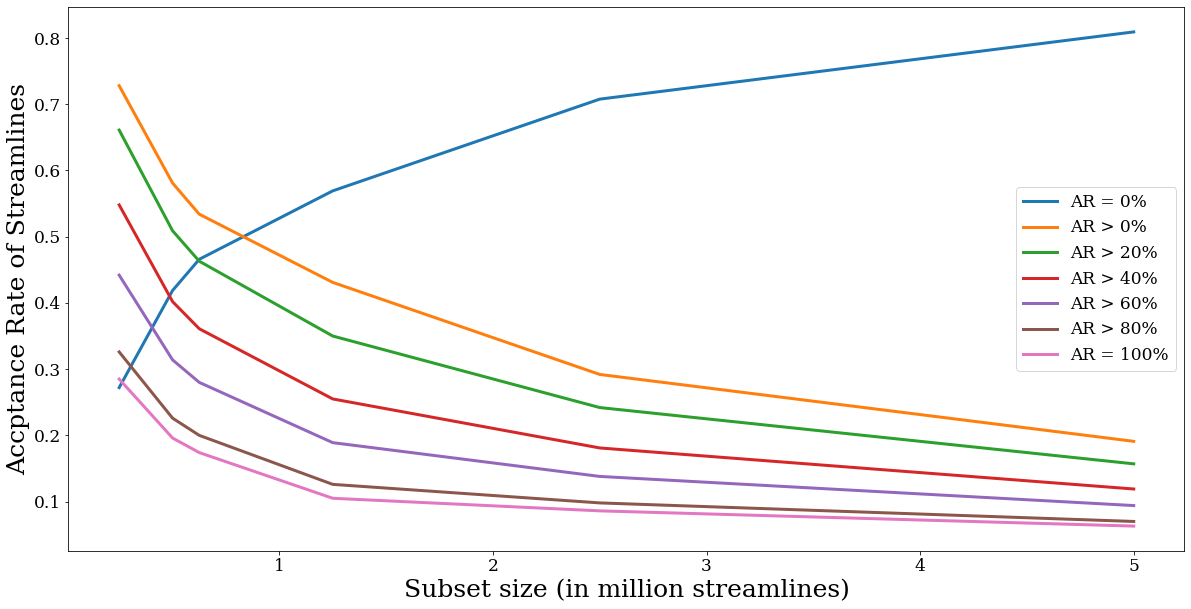
\includegraphics[width= 15cm]{figures/ARplot.png}
        \caption{The changes of acceptance rate from rCOMMIT with different subset size.
        The curves show the averaged AR over subjects. As shown, the ARs of streamlines get higher in the smaller
        subsets.}
    \label{fig:ARplot}
\end{figure}

\begin{figure}[ht]
    \centering
    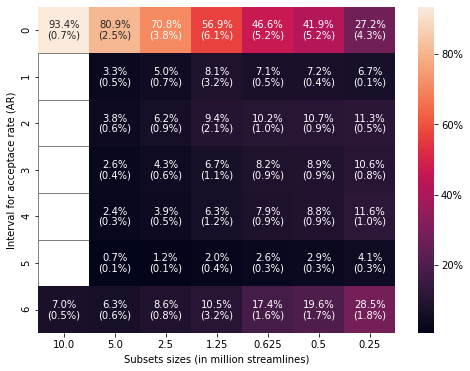
\includegraphics[width= 13cm]{figures/heatmap.png}
        \caption{The distribution of acceptance rates in different subset sizes. Each cell includes the mean ratio of 
        the streamlines across subjects and the standard deviations in the parentheses. In the column of the 10 million data, there is no value from category 1 to 5.
        }
    \label{fig:heatmap}
\end{figure}

The distribution of results between normal COMMIT and rCOMMIT are shown in Fig. \ref{fig:ori_distri} and Fig. \ref{fig:threegroup}.
As shown in the Fig. \ref{fig:ori_distri}, only a small amount of streamlines is kept by COMMIT. As shown in the Fig. \ref{fig:threegroup}, the rCOMMIT influences the distribution of the streamlines and the remaining 
streamlines are mostly among the short ones. The length of rejected streamlines is of higher variety. The distribution of inconclusive streamlines
is similar to the distribution of the input data.

\begin{figure}[ht]
    \centering
    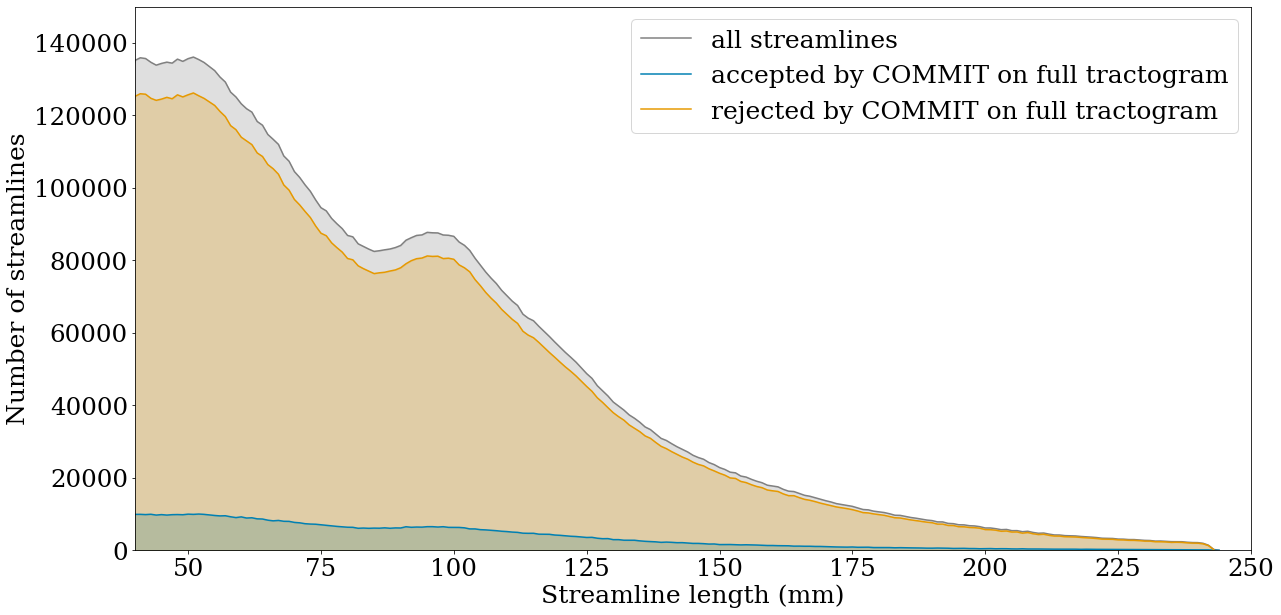
\includegraphics[width= 15cm]{figures/distributon_origi.png}
        \caption{The distribution of streamlines from one exemplary subject filtered by COMMIT. COMMIT is applied on the raw data of 10 million streamlines, which are 
        divided into two groups: rejected and accepted groups.}
    \label{fig:ori_distri}
\end{figure}

\begin{figure}[ht]
    \centering
    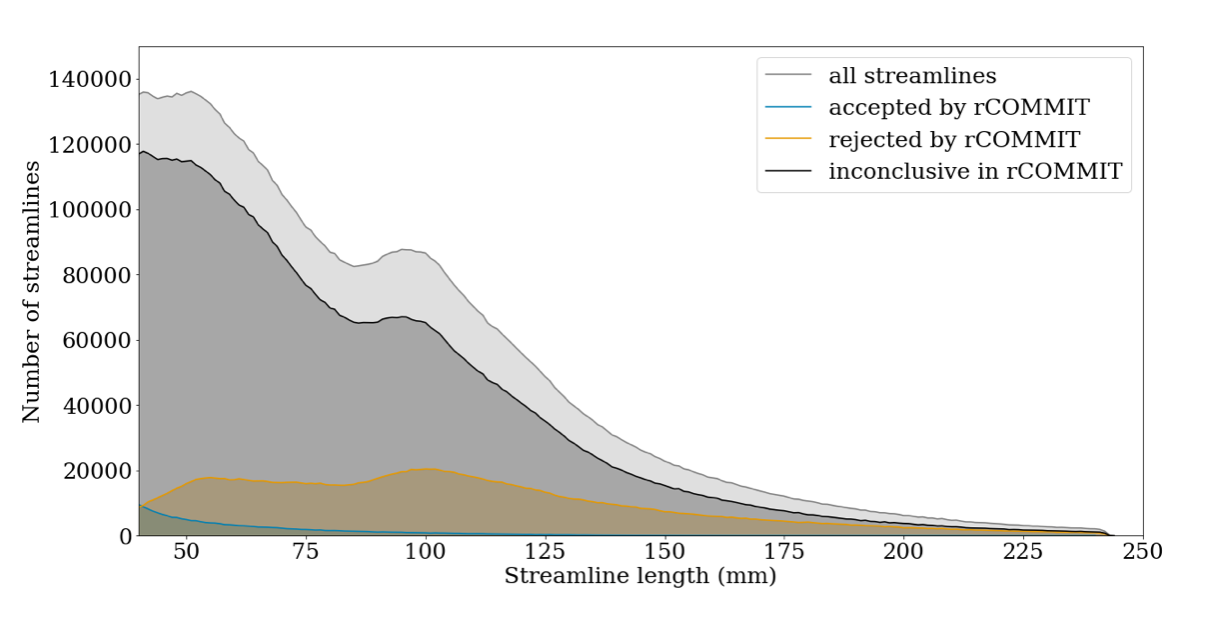
\includegraphics[width= 15cm]{figures/three_groups_hist.png}
        \caption{The distribution of streamlines from one exemplary subject with respect to the length in three groups: plausible group, implausible group and inconclusive group. }
    \label{fig:threegroup}
\end{figure}


With the AR assessments from each size of data, a pseudo ground truth for the subject can be extracted.


\section{Model Classification}

\section{Comparison Between rCOMMIT and rSIFT}

\subsection{Performance between methods}

\subsection{Results from rCOMMIT and rSIFT}

\begin{table}[]
    \centering
    \resizebox{\columnwidth}{!}{%
    \begin{tabular}{|cc|cc|cc|cc|cc|}
    \hline
    \multicolumn{2}{|c|}{Groups} &
      \multicolumn{2}{c|}{Plausible Group} &
      \multicolumn{2}{c|}{Intersection} &
      \multicolumn{2}{c|}{Implausible Group} &
      \multicolumn{2}{c|}{Intersection} \\ \hline
    \multicolumn{2}{|c|}{Methods} &
      \multicolumn{1}{c|}{rCOMMIT} &
      rSITF &
      \multicolumn{1}{c|}{rCOMMIT} &
      rSITF &
      \multicolumn{1}{c|}{rCOMMIT} &
      rSITF &
      \multicolumn{1}{c|}{rCOMMIT} &
      rSITF \\ \hline
    \multicolumn{1}{|c|}{Number of streamlines} &
      \multirow{2}{*}{Subject 1} &
      \multicolumn{1}{c|}{475 959} &
      146 252 &
      \multicolumn{2}{c|}{89 052} &
      \multicolumn{1}{c|}{1 663 161} &
      5 263 290 &
      \multicolumn{2}{c|}{1 486 537} \\ \cline{1-1} \cline{3-10} 
    \multicolumn{1}{|c|}{Percentage} &
       &
      \multicolumn{1}{c|}{4,76 \%} &
      1,46 \% &
      \multicolumn{1}{c|}{18,71 \%} &
      60,89 \% &
      \multicolumn{1}{c|}{16,63 \%} &
      52,63 \% &
      \multicolumn{1}{c|}{89,38 \%} &
      28,24 \% \\ \hline
    \multicolumn{1}{|c|}{Number of streamlines} &
      \multirow{2}{*}{Subject 3} &
      \multicolumn{1}{c|}{215 796} &
      170 814 &
      \multicolumn{2}{c|}{62 376} &
      \multicolumn{1}{c|}{1 970 751} &
      5 445 176 &
      \multicolumn{2}{c|}{1 813 401} \\ \cline{1-1} \cline{3-10} 
    \multicolumn{1}{|c|}{Percentage} &
       &
      \multicolumn{1}{c|}{2,16 \%} &
      1,71 \% &
      \multicolumn{1}{c|}{28,91 \%} &
      36,52 \% &
      \multicolumn{1}{c|}{19,71 \%} &
      54,45 \% &
      \multicolumn{1}{c|}{92,02 \%} &
      33,30 \% \\ \hline
    \multicolumn{1}{|c|}{Number of streamlines} &
      \multirow{2}{*}{Subject 3} &
      \multicolumn{1}{c|}{379 458} &
      176 320 &
      \multicolumn{2}{c|}{88 715} &
      \multicolumn{1}{c|}{2 581 409} &
      5 195 768 &
      \multicolumn{2}{c|}{2 215 674} \\ \cline{1-1} \cline{3-10} 
    \multicolumn{1}{|c|}{Percentage} &
       &
      \multicolumn{1}{c|}{3,79 \%} &
      1,76 \% &
      \multicolumn{1}{c|}{23,38 \%} &
      50,31 \% &
      \multicolumn{1}{c|}{25,81 \%} &
      51,96 \% &
      \multicolumn{1}{c|}{85,83 \%} &
      42,64 \% \\ \hline
    \end{tabular}%
    }
    \end{table}





\begin{figure}[ht]
    \centering
    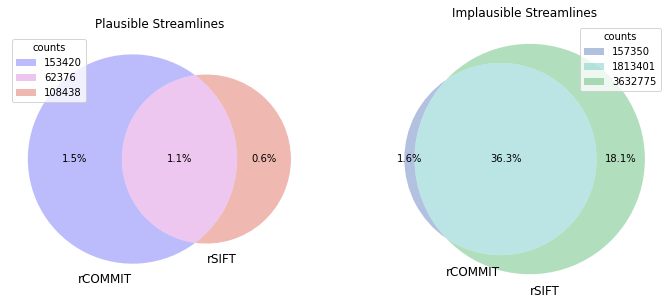
\includegraphics[width= 15cm]{figures/comp_s_c.png}
        \caption{The distribution of streamlines from one exemplary subject with respect to the length in three groups: plausible group, implausible group and inconclusive group. }
    \label{fig:com_s_c}
\end{figure}


Describe the results of the degree project.
